\begin{frame}{Results: Convergence Quality}

\begin{columns}[c]
\begin{column}{0.48\textwidth}
    \begin{block}{Training Convergence}
    \begin{itemize}
        \item Initial loss: \textbf{0.47}
        \item Final loss: \textbf{0.36}
        \item Perplexity: \textbf{1.30-1.32}
        \item Comparable to BF16
    \end{itemize}
    \end{block}

    \vspace{0.3cm}

    \begin{block}{Convergence Characteristics}
    \begin{itemize}
        \item Smooth loss curve
        \item No divergence issues
        \item Stable throughout training
        \item Maintained model quality
    \end{itemize}
    \end{block}
\end{column}

\begin{column}{0.50\textwidth}
    \centering
    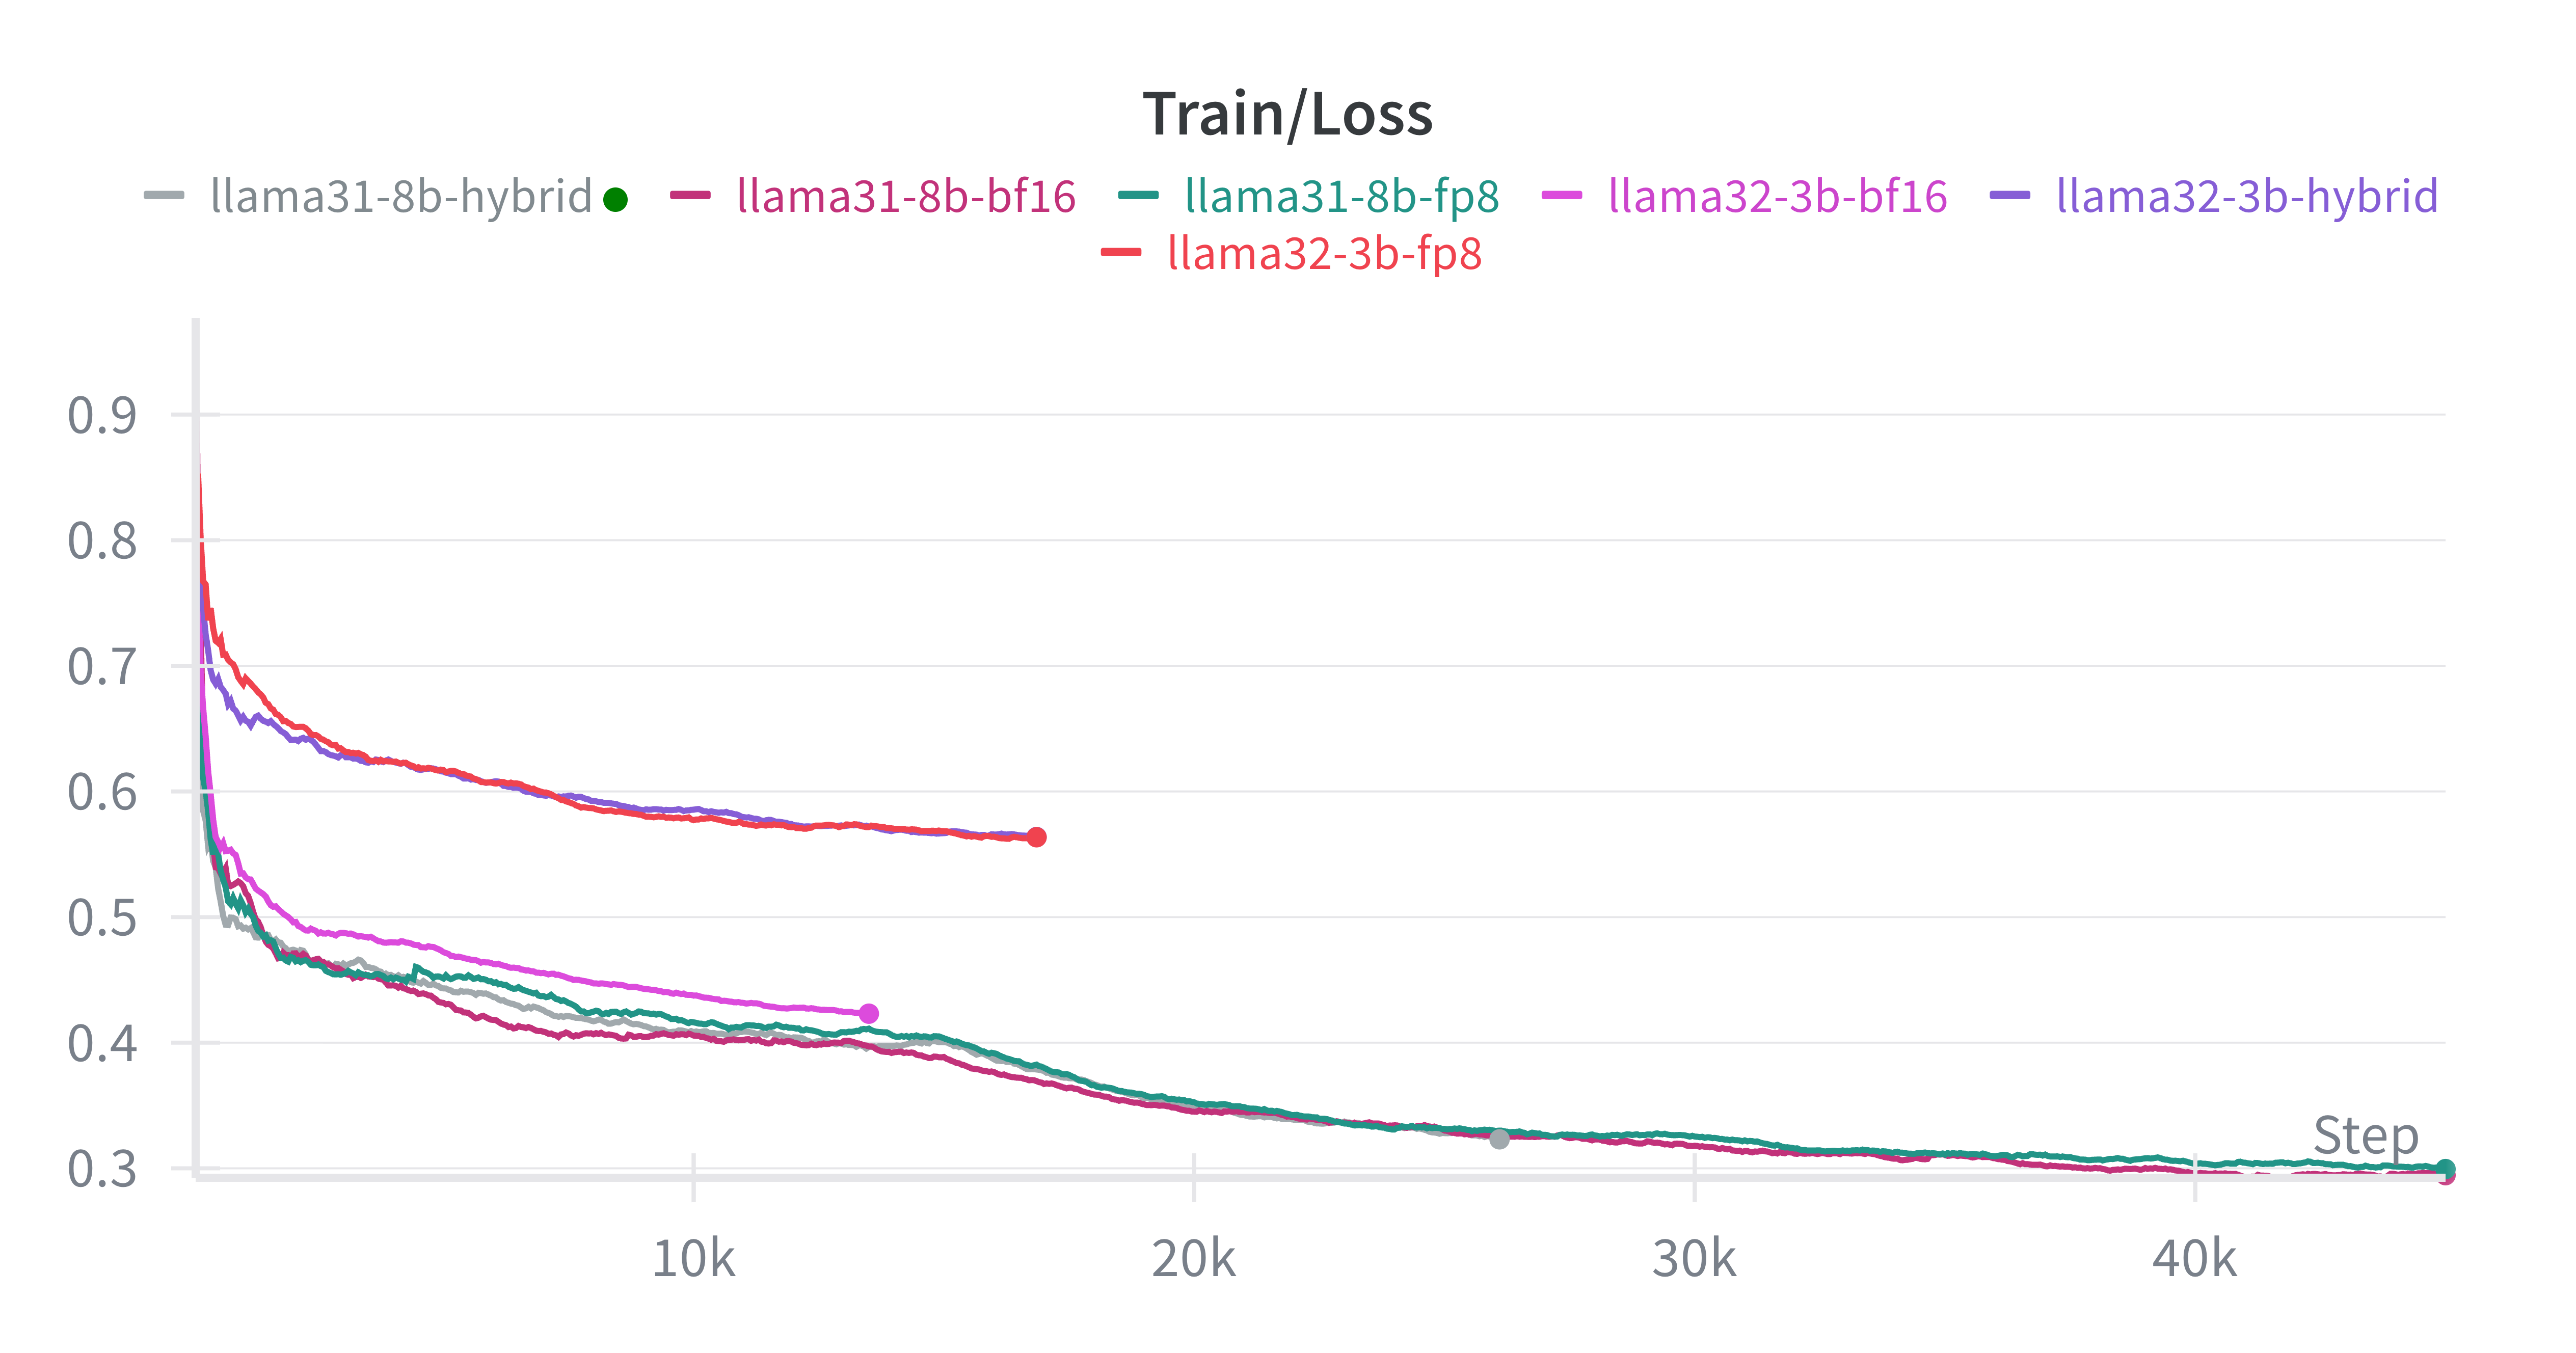
\includegraphics[width=\textwidth]{figures/avg_loss.png}

    \vspace{0.3cm}

    \small
    \textbf{Key Finding:} Layer-wise FP8 achieves comparable final loss and perplexity to BF16 baseline with smoother training dynamics.
\end{column}
\end{columns}

\end{frame}
